\documentclass[0-protokol.tex]{subfiles}
\begin{document}

Tranzistor je polovodičová součástka složená ze dvou PN přechodů se třemi elektrodami - emitor, kolektor a báze. V tomto praktiku měříme vlastnosti tranzistoru se společným emitorem NPN.

Vstupní charakteristika tranzistoru je funkční závislost proudu tekoucího bází na napětí mezi bází a emitorem,
\begin{equation}
I_{BE} = f(U_{BE}),
\end{equation}
výstupní charakteristika je závislost proudu tekoucího kolektorem na napětí mezi kolektorem a emitorem,
\begin{equation}
I_{CE} = f'(U_{CE}). 
\end{equation}
Typické průběhy obou jsou uvedeny v \cite{stud_text}, tyto závislosti měříme pomocí zapojení \ref{fig:zap_u12}.

\begin{figure}[H]
\centering
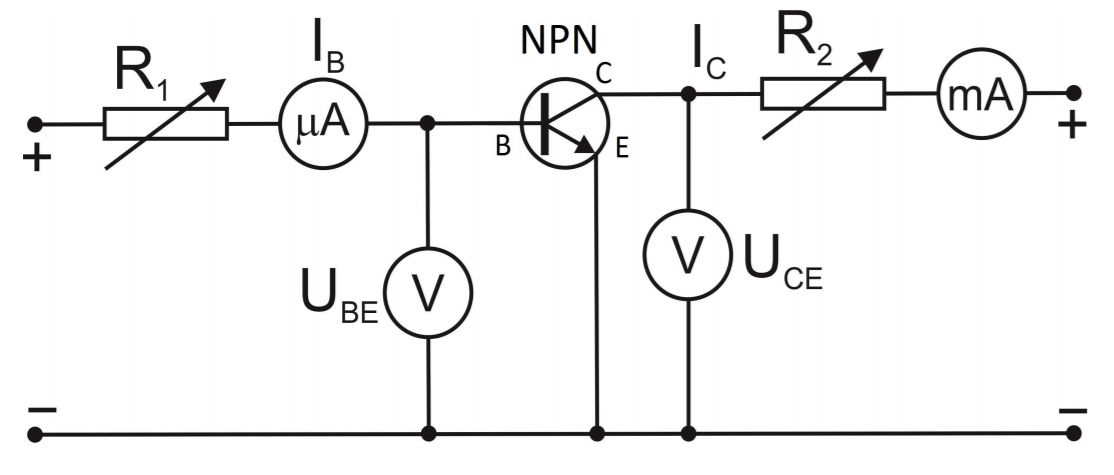
\includegraphics[scale=0.55]{zap_u12}
\caption{Zapojení použité pro úkol 1 a 2}
\label{fig:zap_u12}
\end{figure}

V zapojení se společným emitorem funguje tranzistor jako zesilovač proudu. Přivedení malého proudu na bázi se projeví tokem většího proudu v kolektorovém obvodu. Toto zesílení je popsáno činitelem proudového zesílení $\beta$,
\begin{equation}
\beta = \left(\frac{\Delta I_{CE}}{\Delta I_{BE}}\right)_{U_{CE} = \text{konst.}}.
\end{equation}
Tento činitel získáme lineární regresí závislosti $I_{CE}$ na $I_{BE}$ měřené pomocí \ref{fig:zap_u3}.

\begin{figure}[H]
\centering
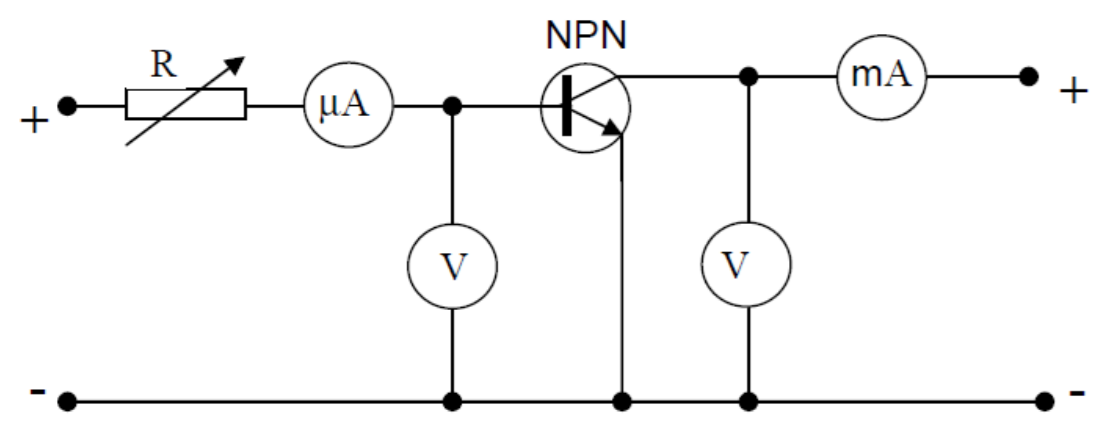
\includegraphics[scale=0.55]{zap_u3}
\caption{Zapojení použité pro úkol 3}
\label{fig:zap_u3}
\end{figure}

\end{document}
